Adesso teniamo conto delle perturbazioni che l'orbita del satellite subisce,
andando quindi a calcolare la risposta forzata, considerando la non sfericità
della Terra e la presenza delle forze non gravitazionali. Vi sono diversi tipi
di orbite che possono essere realizzate, nel nostro caso l'orbita sarà
elio-sincrona, quindi i raggi solari andranno a colpire sempre la stessa faccia
del satellite. Poiché la direzione Sole-Terra ruota per tutta la durata
dell'anno solare, il piano orbitale non può rimanere fisso nello spazio, ma la
linea dei nodi deve ruotare, introducendo così il moto di precessione. Per fare
ciò bisogna far ruotare l'asse dei nodi per mantenere il piano orbitale sempre
con lo stesso angolo ripetto la direzione Sole-Terra
\begin{equation}
\omega_s\approx \frac{2\pi}{365.25\times86400}\approx 0.2 \ \mu rad/s
\end{equation}
Un'orbita di questo tipo è non kepleriana, ma possiamo sfruttare le
perturbazioni esterne per assicurarci il moto di precessione. Si può dimostrare
che grazie alll'appiattimento terrestre, ad una specifica inclinazione del piano
orbitale, dipendente dall'eccentricità e dalla lunghezza del semi-asse maggiore,
il moto di precessione viene perseguito in maniera naturale. Considerando il
nostro caso, ovvero un'orbita ad una bassa altitudine e una piccola eccentricità
e considerando la costante $J_2$, definita come la seconda armonica zonale (essa
rappresenta l'appiattimento ai poli del globo terrestre), per assicurarci il
moto di precessione l'orbita dev'essere di tipo quasi-polare.
Come accennato in precedenza è necessario tenere conto di ogni causa che può
modificare l’orbita del satellite. I principali fattori di cui tenere conto
sono: le anomalie del campo gravitazionale, le forze elettromagnetiche, e le
forze aerodinamche o di attrito. Focalizzeremo l'attenzione sulle forze
di attrito (drag forces), ovvero le perturbazioni causate dalle molecole
dell'atmosfera rarefatta. Azzerare queste perturbazioni è lo scopo del controllo
drag-free.
In base alle proprietà della superficie del satellite, inclusa la sua
temperatura, le molecole dell'atmosfera incidono su di essa in due differenti
modi, figura \ref{fig:riflessione}
\begin{itemize}
  \item Riflessione speculare (o elastica), avviene quando le molecole
  rimbalzano sulla superficie senza perdita di energia, ciò implica che la
  velocità di uscita delle molecole $\vec{v_0}$ è complanare alla velocità
  $\vec{-v_r}$ con la quale impattano la superficie e gli angoli di incidenza e
  di riflessione sono uguali
\begin{equation}
\begin{array}{l}
\vec{v_r}=v_r(\cos{\alpha \vec{n}}-\sin{\alpha \vec{t}}) \\
\Delta \vec{v_s}=((\vec{-v_r}\vec{-v_r})\vec{n})\vec{n} +
((\vec{-v_r}\vec{+v_r})\vec{t})\vec{t} = -2v_r\cos{\alpha \vec{n}}
\end{array}
\end{equation}
  \item Riflessione diffusa (o termica), si ha quando le particelle chi
  colpiscono la superficie perdono tutta la loro energia nell'impatto.
  L'assorbimento delle molecole dipende dalla temperatura della superficie del
  satellite
\begin{equation}
\begin{array}{l}
\vec{v_d}=v_d(\theta_s)\vec{n} \\
\Delta\vec{v_d}=((\vec{-v_d}\vec{-v_r})\vec{n})\vec{n} +
((\vec{-v_d}\vec{-v_r})\vec{t})\vec{t}
= -(v_r\cos{\alpha}+v_d)\vec{n}-v_r\sin{\alpha}\vec{t}
\end{array}
\end{equation}
\end{itemize}

\begin{figure}[htp]
\begin{center}
  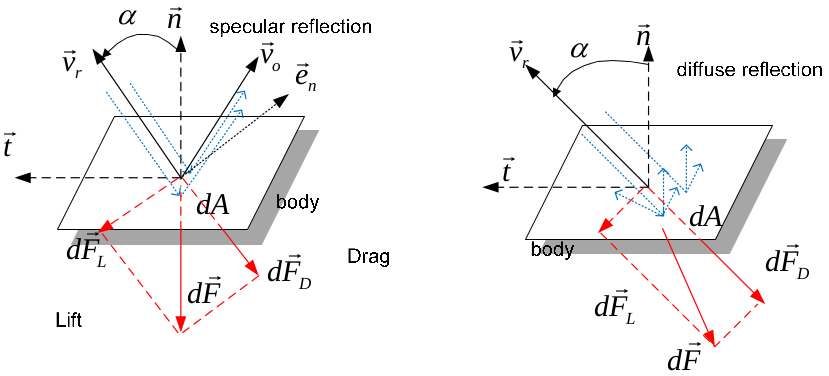
\includegraphics[width=\textwidth]{modelling/orbit_dynamics/image/riflessione.png}
  \caption{Riflessione speculare e diffusa su di una superficie}
  \label{fig:riflessione}
\end{center}
\end{figure}


%2) Diffuse (or thermal) reflection, when the particles hitting the surface lose
% all energy, and 2
%they may leave the surface with a kinetic energy per unit mass 0.5vd depending
% on the surface temperature θ s through the ideal gas law (3.100), now written as
%2
%0.5vd = Rθ s / M a . Molecular re-emission may occur in any direction, but in
% the average [4] the momentum per unit mass aligns with the surface normal, i.e. vd = vd (θ s ) n , which
%now implies a momentum exchange including a tangential component as follows
%Δvd = ( ( −vd − vr ) ⋅ n ) n + ( ( −vd − vr ) ⋅ t ) t = − ( vr cos α + vd ) n −
% vr sin α t .
